\documentclass[10pt, french, a4paper]{report}

\usepackage{babel}
\usepackage{fontspec}
\usepackage{graphicx}
\usepackage{titlesec}
\usepackage{tikz}
\usepackage{uml}
\usepackage[hidelinks]{hyperref}
\usepackage{appendix}
\usepackage{amsmath}
\usepackage{todonotes}

\newfontfamily{\codefont}{JetBrains Mono}[Scale=0.85]
\setmainfont[Ligatures={TeX, Common, Rare, Historic}]{Linux Libertine}

\newcommand{\class}[1]{{\codefont \NoAutoSpacing \mbox{#1}}}

\titleformat{\chapter}
	{\normalfont\LARGE\bfseries}{\thechapter.}{1em}{}

\tikzset{every picture/.style={execute at begin picture={
   \NoAutoSpacing;}
}}


\renewcommand\appendixtocname{Annexes}

\title{
	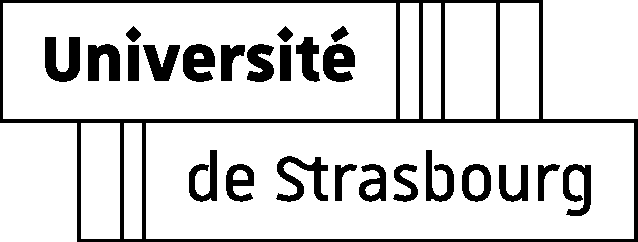
\includegraphics[width=0.5\textwidth]{logo-uds.pdf}\\
	\vspace{2em}
	Master~1 -- Image et 3 Dimensions\\
	Projet de Programmation Avancée\\
	Rapport Final
}
\author{Maxime \textsc{Hohl}}
\date{\today}


\begin{document}

\maketitle

\tableofcontents

\chapter{Design}

Le jeu \textit{Asteroids} est découpé en deux grandes parties, le moteur et le jeu lui 
même. Le moteur est lui même découpé en 3 modules~:
\begin{itemize}
	\item Le module de rendu~: s'occupe de l'affichage de différents éléments à l'écran.
	\item Le module de physique~: S'occupe des calculs physique, c'est à dire des
	      déplacements et des collisions.
	\item Le module de GUI~: S'occupe de l'affichage des éléments d'interface utilisateur.
	\item Le module de particules~: Un système de particules qui ne fonctionne pas encore 
	      dans la version rendue, bien qu'il soit assez avancé d'un point de vue du 
	      développement.
\end{itemize}
Voir la Figure~\ref{fig:design-global}.

Tout les éléments du jeu et du moteur interagissent ensemble grâce au \textit{design pattern} Observateur.

\begin{figure}[h]
	\center
	\caption{Design global}
	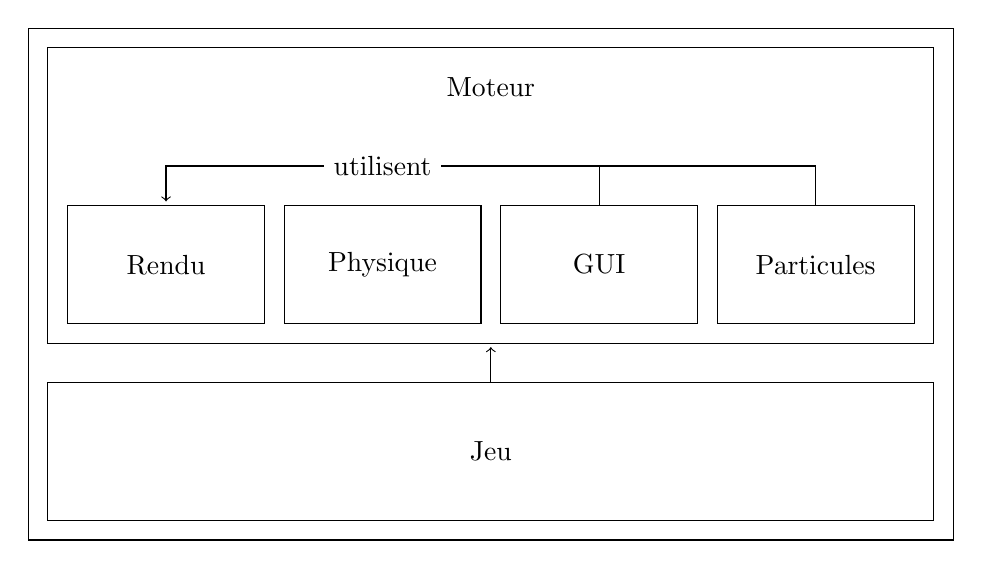
\begin{tikzpicture}	
		\draw (0, 0) rectangle (11.75, 6.5);
	
		
		\draw (0.25, 2.5) rectangle (11.5, 6.25);
		\node at (5.875, 5.75) {Moteur};
		
		\draw (.5, 2.75) rectangle (3, 4.25);
		\node at (1.75, 3.5) {Rendu};
		
		\draw (3.25, 2.75) rectangle (5.75, 4.25);
		\node at (4.5, 3.5) {Physique};
		
		\draw (6, 2.75) rectangle (8.5, 4.25);
		\node at (7.25, 3.5) {GUI};
		
		\draw (8.75, 2.75) rectangle (11.25, 4.25);
		\node at (10, 3.5) {Particules};

		\node (utilise) at (4.5, 4.75) {utilisent};		
		\draw[->] (7.25, 4.25) -- (7.25, 4.75) 
				  -- (utilise) 
				  -- (1.75, 4.75) -- (1.75, 4.30);
		\draw (10, 4.25) -- (10, 4.75) -- (7.25, 4.75);


		\draw (.25, .25) rectangle (11.5, 2);
		\node at (5.875, 1.125) {Jeu};
		
		\draw[->] (5.875, 2) -- (5.875, 2.45);
	\end{tikzpicture}
	\label{fig:design-global}
\end{figure}

\section{Le \textit{design pattern} Observateur}

Ce \textit{design pattern} permet la communication entre les différents éléments du
jeu. Il est composé d'éléments appelés \textit{Observer} qui vont \og recevoir \fg{} 
les messages envoyés par les éléments \textit{Subject} qu'ils observent.

Cf. L'article Wikipedia pour plus d'informations~: 
\url{https://en.wikipedia.org/wiki/Observer_pattern}.

\section{Le module de rendu}

Le module de rendu s'occupe de l'affichage de tout les éléments à l'écran. Il est basé
sur la bibliothèque \textit{SDL2} mais à était conçu pour pouvoir changer très facilement, 
par \textit{OpenGL} ou \textit{Vulkan} par example.

Il propose des fonctions de base permettant d'afficher tout les éléments simples 
suivants~:
\begin{itemize}
	\item Des Points
	\item Des Lignes
	\item Des Rectangles vides et pleins
	\item Des polygones quelconques vide
	\item Des Cercle
\end{itemize}

Les modules de GUI et de particules se basent sur lui.

\section{Le module de physique}

Le module de physique s'occupe de tout les calculs physique, c'est à dire, en l'état
actuel des choses, des déplacements en utilisant accélération, vitesse et position 
ainsi que des collisions cercles-cercles, point-cercle et joueur-cercle, le joueur
étant un polygon quelconque et bien définis.


\section{Le module de GUI}

Le module de GUI s'occupe de la gestion de tout les éléments d'interface graphique.
En l'état actuel il permet de gérer~:
\begin{itemize}
	\item Des \textit{Panels}~: qui sont de simples rectangles.
	\item Des textes~: qui, aussi surprenant que ça puisse paraitre, sont du texte.
\end{itemize}

Le module à était conçu pour permettre l'ajout de nouveaux éléments d'interface de 
manière assez facile. 

\section{Le module de système de particules}

Ce module ne fonctionne pas encore, mais comme le gros est déjà développé et que, 
personnellement, je le trouve plutôt réussi, je l'ai quand même ajouté au code, bien
qu'il ne soit actuellement pas utilisé par le jeu.

Il permet de gérer des particules de type point, avec un couleur spécifique.

\section{Le jeu}

Le jeu permet de gérer les astéroïdes au fur et à mesure du temps et en fonction 
du score du joueur. 
Le joueur gagne un point par astéroïde détruit. 

Tout les éléments du jeu reposent sur les différents modules du moteur.


\chapter{Implantation}

L'implantation se s'est faite de manière très directe avec design décrit précédemment.

Pour le digramme UML du code du projet, voir Annexe~\ref{chap:digramme-uml}.

\section{Le \textit{design pattern} Observateur}

Toutes les \textit{class} qui veulent échanger des donnés doivent hériter de la 
\textit{class} \class{Subject} quand elles transmettent des donnés ou de la 
\textit{class} \class{Observer} quand elles reçoivent des donnés. Ces deux \textit{class} on comme paramètre de template le type de donné échangé.

\section{Le module de rendu}

Le module de rendu est constitué d'une \textit{class} appelée \class{Renderer} qui 
se base sur \textit{SDL2} mais qui permet de changer aisément pour tout autre 
système en arrière-plan, comme \textit{OpenGL}, \textit{Vulkan}, \textit{Metal}, etc. 


\section{Le module de physique}

Le module de physique est axé sur deux \textit{class} principales, 
\class{PhysicEngine} et \\ \class{PhysicEntity}. 
La première effectue tout les calculs liés à la physique et 
tous les objets qui doivent êtres inclus dans les calculs physiques doivent hériter
de la seconde.

Le calcul des mouvements des objets se basent sur les trois formules simples suivantes,
avec $a$ l'accélération, $v$ la vitesse et $r$ la position~:
\begin{align}
	a_t &= a_0\\
	v_t &= v_{t-1} + a_t * \Delta t\\
	r_t &= r_{t-1} + v_t * \Delta t
\end{align}
Avec $a_0$, $v_0$ et $r_0$ défini.

Le système de collision ne permet actuellement que de détecter des collisions du type
cercle-cercle, cercle/point et cercle/joueur.

Les collisions cercles/joueur sont gérés de manière assez particulières. 
Le joueur est un polygone concave quelconque (voir Figure~\ref{fig:model-joueur}), 
il faudrait donc utiliser un algorithme d'intersection entre cercle et polygone concave,
mais ces algorithmes sont assez complexes à mettre en place, et en observant bien la 
forme do polygone joueur et la différence de taille entre le joueur et les cercles 
(ici, les astéroïdes), on se rend compte que l'on peut tout simplement effectuer un 
test de collision entre le cercle et les trois points \og extérieurs \fg{} (en rouge sur la Figure~\ref{fig:model-joueur}) du polygone et si un point est dans un cercle
alors il y a collision entre cercle et joueur.

\begin{figure}[h]
	\center
	\caption{Le polygone du joueur}
	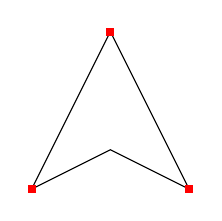
\begin{tikzpicture}[scale=-.5]
		\draw (0, -2) -- (2, 2) -- (0, 1) -- (-2, 2) -- cycle;
		\fill[red] (-0.1, -2.1) rectangle (0.1, -1.9);
		\fill[red] (1.9, 1.9) rectangle (2.1, 2.1);
		\fill[red] (-2.11, 1.9) rectangle (-1.9, 2.1);
	\end{tikzpicture}
	\label{fig:model-joueur}
\end{figure}

\todo[inline]{Correctement positionner les points rouge} 


\section{Le module de GUI}

Le module de GUI tourne autour des \textit{class}~:
\begin{itemize}
	\item \class{gui::Gui} qui est la \textit{class} de base de gestion des 
	      éléments d'interface. C'est elle qui gère le rendu et qui doit être
	      utilisée pour créer tout les éléments d'interface.
	\item \class{gui::Entity} qui est la \textit{class} virtuelle pure dont tout
		  les éléments d'interface doivent hériter.
\end{itemize}

Chaque entité est positionnée relativement à son parent et à son ancrage. 
Les entités sans parent sont placées par rapport à la fenêtre, toujours en fonction
de l'ancrage (voir Figure~\ref{fig:gui-positionement}).

\begin{figure}[h]
	\center
	\caption{Le positionnement des éléments d'interface. Chaque élément est représenté avec son point d'ancrage. Les éléments vert et rouge ont pour parent l'élément blue, et ce dernier à pour parent la fenêtre (en noir).}
	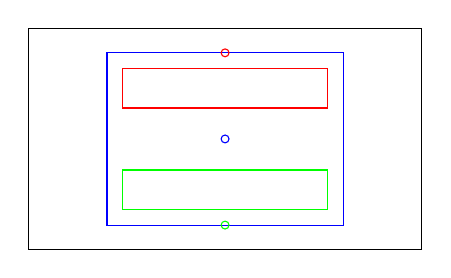
\begin{tikzpicture}		
		\draw (0, 0) rectangle (5, 2.8125);
		
		\draw[blue] (1, .3125) rectangle (4, 2.5);
		\draw[blue] (2.5, 1.40625) circle (0.05cm);
		
		\draw[green] (1.2, .5125) rectangle (3.8, 1.0125);
		\draw[green] (2.5, .3125) circle (0.05cm);
		
		\draw[red] (1.2, 1.8) rectangle (3.8, 2.3);
		\draw[red] (2.5, 2.5) circle (0.05cm);
		
	\end{tikzpicture}
	\label{fig:gui-positionement}
\end{figure}

Chaque entité va se dessiner en appelant des fonctions de la \textit{class} 
\class{GUIRenderer} puis appeler la fonction de rendu de ses enfants.
Donc si l'on se représente les éléments d'interface via un arbre grâce à leur
lien de parenté, le rendu se fait dans un ordre de parcoure en profondeur, ce
qui permet de garantir que les parents sont toujours rendus avant leur enfants (et donc sont affichés derrière). Voir Figure~\ref{fig:gui-ordre-rendu}.

\begin{figure}[h]
	\center
	\caption{Ordre de rendu des éléments graphiques
			 (le numéro représentant l'ordre d'affichage)}
	\begin{tikzpicture}[]
		\node{Root}
			child { node {1} 
				child { node {2} }
				child { node {3} }
			}
			child { node {4} }
			child { node {5} 
				child { node {6} 
					child { node {7} }
					child { node {8} }
				}
				child { node {9} }
			};
	\end{tikzpicture}
	\label{fig:gui-ordre-rendu}
\end{figure}

Ce module est le plus aboutit de tous, il ne dispose pas de beaucoup d'éléments
différents, mais il conçu de tel sorte qu'en ajouter un est extrêmement aisé.
Il suffit de créer une \textit{class} qui hérite de \class{gui::Entity} 

\section{Le module de système de particules}

\todo[inline]{A faire}

\section{Le jeu}

Le jeu en lui même est axé autour des trois \textit{class} suivantes~:
\begin{itemize}
	\item \class{Game}~: qui gère toute la logique du jeu, c'est à dire la boucle
		  principale, les appels de rendu, la gestion des évènements la créations
		  des différents éléments du jeu, etc.
	\item \class{Player}~: qui gère toute la logique derrière le joueur, c'est à dire
		  ses déplacements, et ses tirs.
	\item \class{Asteroids}~: qui gère tout les astéroïdes, de leur création au cours
		  du temps et en fonction du score du joueur à leur destruction si ils sont
		  touchés par des tirs du joueur. 
\end{itemize}


\chapter{Problèmes}

\todo[inline]{A faire}

\appendix
\addappheadtotoc

\chapter{Diagramme UML du Projet}
\label{chap:digramme-uml}

\todo[inline]{A faire}

\umlDiagram[box=,border,sizeX=7cm,sizeY=4cm]{%
	\umlClass[refpoint=bl, pos={3,3}]{ClassName}{}{}}

\end{document}
